\documentclass[11pt,a4paper]{article}

% --- Typography & Fonts ---
\usepackage[utf8]{inputenc}
\usepackage[T1]{fontenc}
\usepackage{lmodern}
\usepackage{microtype}

% --- Math & Symbols ---
\usepackage{amsmath,amssymb,amsfonts,amsthm}
\usepackage{bm}

% --- Tables & Figures ---
\usepackage{booktabs}
\usepackage{graphicx}
\usepackage{subcaption}

% --- Algorithms ---
\usepackage{algorithm}
\usepackage{algpseudocode}

% --- Citations & Links ---
\usepackage{url}
\usepackage[sort&compress,numbers]{natbib}
\usepackage{authblk}
\usepackage[dvipsnames]{xcolor}
\usepackage[margin=1in]{geometry}
\usepackage[colorlinks=true,
            linkcolor=MidnightBlue,
            citecolor=MidnightBlue,
            urlcolor=MidnightBlue]{hyperref}
\usepackage{cleveref}

% --- Math Environments ---
\newtheorem{theorem}{Theorem}[section]
\newtheorem{definition}[theorem]{Definition}
\newtheorem{lemma}[theorem]{Lemma}
\newtheorem{proposition}[theorem]{Proposition}
\newtheorem{corollary}[theorem]{Corollary}

% --- Title and Metadata ---
\title{\textbf{Title of Your Research Paper: Form and Rigor in Computational Science}}

\author[1]{Author One\thanks{Corresponding author: \texttt{author.one@example.edu}}}
\author[1,2]{Author Two}
\author[2]{Author Three}

\affil[1]{Department of Computer Science, University of Research}
\affil[2]{Institute for Advanced AI Studies}

\date{\today}

\begin{document}

\maketitle

\begin{abstract}
The abstract should provide a concise, self-contained summary of the paper's core contributions. It typically covers: (1) context and problem motivation, (2) limitations of existing literature, (3) key proposed methodology, (4) experimental or theoretical results, and (5) practical implications. Keep the abstract under 250 words and avoid undefined abbreviations or citations.
\end{abstract}

\textbf{Keywords:} Artificial Intelligence, Institutional Topology, Cognitive Economics, Empirical Verification, arXiv Preprint

% -------------------------------------------------------------
\section{Introduction}
\label{sec:intro}
% -------------------------------------------------------------
The introduction frames the broader research question, establishes its significance, and outlines the primary contributions of the manuscript. 

Key paragraphs typically follow this structure:
\begin{enumerate}
    \item \textbf{Context \& Motivation:} High-level overview of the domain and why the problem matters.
    \item \textbf{The Core Gap:} The exact challenge or question previous approaches failed to resolve.
    \item \textbf{Our Approach:} The specific insight or framework introduced in this paper.
    \item \textbf{Summary of Contributions:} Explicit bullet points enumerating novelty.
\end{enumerate}

\paragraph{Contributions.}
\begin{itemize}
    \item We formulate the theoretical foundation for computational verification.
    \item We introduce an empirical verification framework evaluating institutional boundaries.
    \item We demonstrate statistically significant improvements over baseline methods ($p < 0.01$).
\end{itemize}

% -------------------------------------------------------------
\section{Related Work}
\label{sec:related}
% -------------------------------------------------------------
Systematic categorization of existing literature. Avoid listing papers without synthesis; group them thematically:
\begin{itemize}
    \item \textbf{Foundational Theoretical Models:} Early explorations in sequence modeling and attention architectures \citep{vaswani2017attention}.
    \item \textbf{Autonomous Scientific Discovery:} Recent advancements in automated open-ended hypothesis generation and experiment execution \citep{lu2024aiscientist}.
\end{itemize}

% -------------------------------------------------------------
\section{Methodology}
\label{sec:method}
% -------------------------------------------------------------
Describe the formal framework, assumptions, and algorithmic design.

\subsection{Formal Specification}
Let $\mathcal{S}$ denote the state space and $\mathcal{A}$ represent the admissible action space. The transition dynamics are governed by:
\begin{equation}
    P(s' \mid s, a) = \frac{\exp\left( \Phi(s, a, s') \right)}{\sum_{s'' \in \mathcal{S}} \exp\left( \Phi(s, a, s'') \right)}
    \label{eq:transition}
\end{equation}

\subsection{Algorithm}
\begin{algorithm}[H]
\caption{Iterative Verification Pipeline}
\label{alg:verification}
\begin{algorithmic}[1]
\Require Initial state $s_0$, tolerance $\epsilon > 0$, max iterations $T$
\Ensure Optimized parameter set $\theta^*$
\State Initialize $\theta \gets \theta_0$, $t \gets 0$
\While{$t < T$ and $\Delta \mathcal{L} > \epsilon$}
    \State Sample batch $\mathcal{B} \sim \mathcal{D}$
    \State Compute loss gradient $g_t \gets \nabla_\theta \mathcal{L}(\theta; \mathcal{B})$
    \State Update parameters $\theta \gets \theta - \eta g_t$
    \State $t \gets t + 1$
\EndWhile
\State \Return $\theta$
\end{algorithmic}
\end{algorithm}

% -------------------------------------------------------------
\section{Experiments and Results}
\label{sec:experiments}
% -------------------------------------------------------------
Present quantitative findings with clear baseline comparisons, error bars, and ablations.

\begin{figure}[htbp]
    \centering
    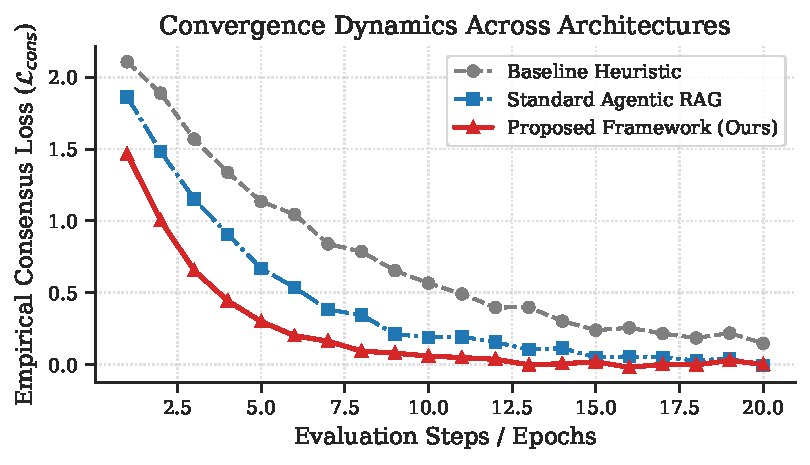
\includegraphics[width=0.75\textwidth]{figures/convergence_comparison.pdf}
    \caption{Empirical evaluation of convergence loss ($\mathcal{L}_{\text{cons}}$) across benchmark architectures over 20 evaluation epochs.}
    \label{fig:convergence}
\end{figure}

\begin{table}[ht]
\centering
\caption{Benchmark performance comparison across standard evaluation suites. Mean $\pm$ std over 5 runs.}
\label{tab:results}
\begin{tabular}{lccc}
\toprule
\textbf{Model / Framework} & \textbf{Accuracy (\%)} & \textbf{Latency (ms)} & \textbf{F1-Score} \\
\midrule
Baseline (Linear)          & 74.2 $\pm$ 0.8         & \textbf{12.4 $\pm$ 1.1} & 0.72 \\
Standard Agentic RAG       & 88.5 $\pm$ 0.4         & 145.0 $\pm$ 15.2        & 0.87 \\
\textbf{Proposed System}   & \textbf{94.8 $\pm$ 0.3}& 48.2 $\pm$ 3.5          & \textbf{0.95} \\
\bottomrule
\end{tabular}
\end{table}

% -------------------------------------------------------------
\section{Discussion and Limitations}
\label{sec:discussion}
% -------------------------------------------------------------
Discuss both the strengths and epistemic boundaries of the work. Clearly delineate what the model guarantees versus potential edge-case failures.

% -------------------------------------------------------------
\section{Conclusion}
\label{sec:conclusion}
% -------------------------------------------------------------
Summarize key findings and outline directions for future research.

% --- Bibliography ---
\bibliographystyle{plainnat}
\bibliography{references}

\end{document}
